\section{Broader impact and outreach}

The best outreach program should be able to easily reach women and
minority groups underrepresented in science. Video games provide
a good way to do just that- a  study from the  Pew Internet 
\& American Life 
Project (Lenhart 2008) found that the percentage of American youth
that play video games is almost the same for a wide range of racial and
ethnic groups and incomes. The survey combined the telephone responses 
from a nationally representative sample of 1,102 young people, ages 12 to 
17, and their parents. It found that 99\% of boys and 94\% of girls
play video games, and they play them often, with  half of the respondents 
saying they had played a video game the previous day. This adds up to
over 200 million person-hours of video gaming each day in the U.S.

Games are clearly entertaining as judged by their use, 
but what if they had educational benefits? 
Our proposal 
focuses not on general computer and video games, but on educational games,
and the ideas we incorporate are 
grounded in a theory of intrinsically motivating instruction 
based on a rigorous study of educational games 
(Malone 1981, Gee 2003,
Squire 2003, Aldrich 2004, Schell 2008).


Through the medium of  games, our outreach aims are the following:\\
\noindent {\bf (1a)} To introduce  elementary and middle
school students to the length scales relevant
to astronomy, from the Solar system to the large scale structure of the Universe
.\\
\noindent{\bf (1b)}  To introduce school children to the chemical constituents
 of the Universe and how they are distributed on Astronomical scales.\\
\noindent{\bf (1c)} To introduce high school students to the concept
of quasars, the  intergalactic medium and absorption lines.\\
{\bf (2)} To provide an interactive 
learning experience. The best way to learn is
to make it an enjoyable  experience from the start. We do not
however want people to take part necessarily
because they want to learn about these
topics. Being entertained is enough, and familiarity with these topics
will come about through the way the game is designed.\\
{\bf (3)}
To reach the largest audience possible. Given that only small fraction of 
the target audience is familiar with  the above concepts  we take the view 
that 
there is a huge amount to be gained from disseminating even simplified 
knowedge among a number of people which is enormous compared to the usual 
outreach channels (lectures  etc..). The gains of this broader 
impact would be to increase interest in science as a career across 
a desirable demographic.
  

\subsection{Minecraft Astronomy lesson plans}




We propose to make lesson plans for elementary and middle school students to 
learn the size scales of the Universe and understand the elemental content 
of the Universe using the popular game Minecraft. 
Minecraft is akin to digital Lego bricks – players inhabit a 
three-dimensional 
world of blocks with its own unique ecosystem and physical laws. Using 
imagination, 
players build whatever they can dream up by mining resources, combining, 
and placing them to build everything from pickaxes 
to complex and working electrical systems. So far, 100 million people have 
purchased 
the Mac/PC version of the game. 
It is considered a sandbox game, providing nearly limitless opportunities 
to  build. Teachers can buy discounted licenses through MinecraftEdu.com, as 
well as a plug-in to tailor the software to a specific curriculum. 



\begin{figure}%[ht!]
\centering
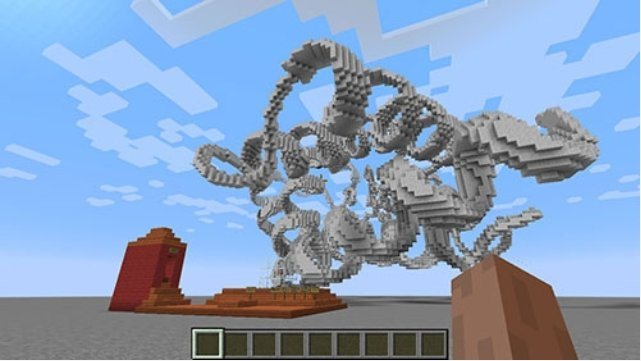
\includegraphics[width=75mm]{figs/myoglobin.jpg}
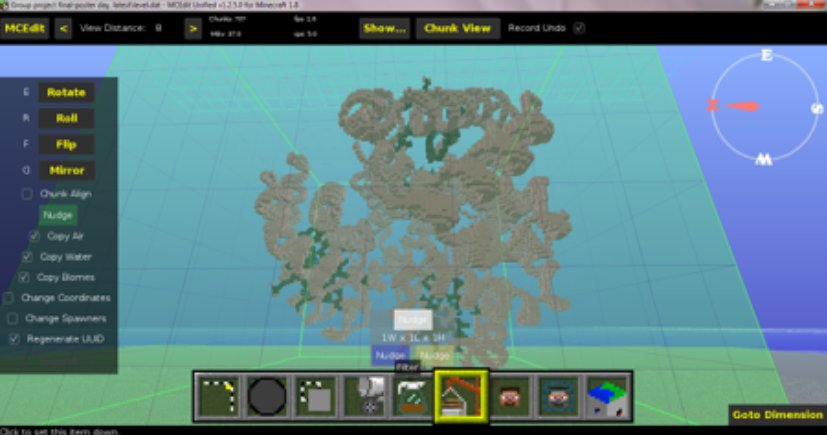
\includegraphics[width=80mm]{figs/mcedit.jpg}
\caption{\footnotesize{{\bf Left:
Minecraft visualization of myoglobin molecule} 
Reproduced from the MolCraft project, University of Hull, UK
{\bf Right: Importing three dimensional structure into Minecraft
using MCedit} Reproduced from the MolCraft project, University of Hull, UK
}}
\label{molcraft}
\end{figure}


As an educational tool, Minecraft teaches design, collaboration, co-creating 
and problem solving. It’s an active learning environment. Previously, 
successful
 physics lessons have been created for studying quantum mechanics 
(q-Craft Curriculum Project) and testing gravity (Rhett Alain, Wired) in 
Minecraft. Gamers enjoy making maps, building things and solving puzzles. 
Our 
Minecraft Astronomy elementary school tutorial will give instructions on 
how to 
build a rocket and how to use it to navigate a map of the Universe hosted 
on our server. Our middle school tutorial will include plans to build a 
telescope and 
how to use it to find the atoms that make up our Universe. Self-driven 
inquiry 
leads to locations on our maps where the content is kept up-to-date.
 Blog 
posts will connect users, guide them in reflective, 
“big picture” 
thought processes, craft intuitive thinking and inspire their natural 
curiosity. 
Astronomy facts, paired with math, cosmic pictures and stories will 
enrich learning.
 
One lesson plan will be primarily for 1st to 4th graders and will focus on the s
ize scale of the solar system.
We have substantial experience in this topic as the PI has been
carrying outreach to this demographic since 2002, as part of the CMU
Physics department's outreach program. Some of the outreach activities
involved making scale models of the solar system with household objects. 
Several limitations can be overcome by using the Minecraft world to do this, 
including  extending the scale of the models arbitrarily, and using the 
3rd dimension.
 A second lesson plan will focus on the atomic content of 
the Universe for middle school students (5th to 7th grade). Game users 
will hunt to  find the rare metals among the hydrogen and helium 
atoms of the universe, finding 
the prized heavy elements in places like rocky bodies and supernovae remnants. 
We will develop worlds based on several different length scales, including
one where we will import galaxy redshift survey data (from the SDSS) so that 
the students can fly around and explore 
the large scale structure of the Universe.
It is simple to import such data sets and edit them- an example
of biological molecules taken 
from the Molcraft project (University of Hull, UK) is shown in Figure 
\ref{molcraft} and it is easy to imagine how astronomical data would work
in this environment.


Overworld dimensions of the square game plane are $3.59 \times 10^{9}$
 square kilometers 
(as compared to the Earth’s spherical $5.09 \times 10^{8}$
 square kilometer area). 
The height  is 256 blocks, but a Sky Dimension of similar size to the 
Overworld is 
planned for a future release. A shared world will be created and gamer guides 
released to aid exploration. For teachers, lesson plans will be made, 
including 
objectives and goals based on educational standards, a prior knowledge test, 
directed instruction, vocabulary definitions, guided practice sets and an assess
ment 
worksheet. As our work progresses, we plan to bring these lessons to a local 
school 
for tests with students.
These include such schools as Colfax School, Milliones School and Helen Faison
academy which we have worked with before, and where there are high fractions
of students from minorities underrepresented in science.
 While these lessons will be available to the 
general public, they will be geared toward educators to be used in classrooms.

\subsection{Universe Sandbox Tutorial}


For high school students, 
we propose using the commercial software Universe Sandbox2 
 (universesandbox.com) to build a Lyman-alpha forest tutorial 
and activity. 
Universe Sandbox is an interactive space simulator, giving players the ability t
o 
wander through sections of the known universe. Universal Sandbox2 is a fully 
featured, space simulator, with new features and simulations added 
based on community requests. Players have the ability to observe and 
change the universe by altering fundamental constants (like the strength of 
gravity) and by moving celestial objects through space and time. 
Our high school and introductory college astronomy lesson will walk 
students through a Lyman-alpha forest simulation to show intervening 
material at differing redshifts. The material creates a forest of absorption 
lines and the tutorial will explain how that is seen in the visual in quasar 
spectra, using diagrams and an interactive applet that allows the students to 
change the density, distance, ionization level and elemental content of the 
intervening material. The users discovery process will be framed as a quest to 
explain the mystery of changes the quasar spectrum, as told in 
comic storyboard 
form following the initial discoveries of Martin Schmidt and Cyril Hazard. 

 

Lectures, books, and video are all linear, and linear media are poor at 
conveying complex systems.  The best way to understand a complex 
system is to play with it, getting a holistic sense of how parts are 
connected.  Such systems that are best learned through simulations 
include the human circulatory system and nuclear reactors. 
In physics, demonstrations and laboratories are all simulations, 
traditionally with physical objects, apparatus, and measuring devices.
The Universe itself is the ultimate complex physical system and arguably
the most exciting one to approach in this way.


